\chapter{Results}
\label{s:results}
Having designed and implemented the gaze tracker, we shall now evaluate its performance.
There are three aspects to consider when talking of performance: robustness, precision and speed.

\section{Face tracking}
In Figure \ref{i:res-face}, we demonstrate the face motion models by fitting a transformation between a pair of images.

The performance of the face tracking methods has not been evaluated in any exact manner because it is difficult to define the ground truth.
We could, for example, evaluate their performance on artificial images not related to faces.
However, that does not evaluate the algorithms---it would be hardly more than a test of the implementation.

\begin{figure}[t]
	\centering 
	\begin{subfigure}[b]{0.55\textwidth}
		\centering 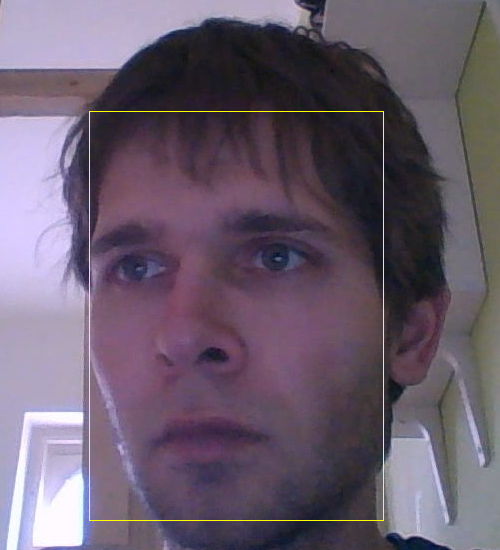
\includegraphics[width=\linewidth]{img/res-face-ref.png} \caption{The reference image.} \label{i:res-face-ref}
	\end{subfigure}
	\begin{subfigure}[b]{0.49\textwidth}
		\centering 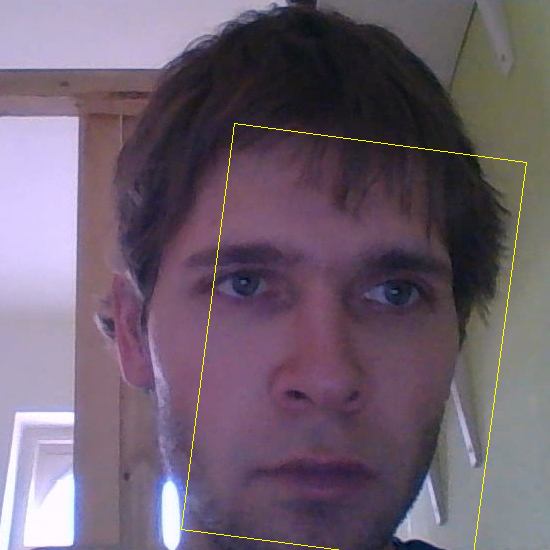
\includegraphics[width=\linewidth]{img/res-face-locrot.png} \caption{Location-rotation tracker.} \label{i:res-face-locrot}
	\end{subfigure}
	\begin{subfigure}[b]{0.49\textwidth}
		\centering 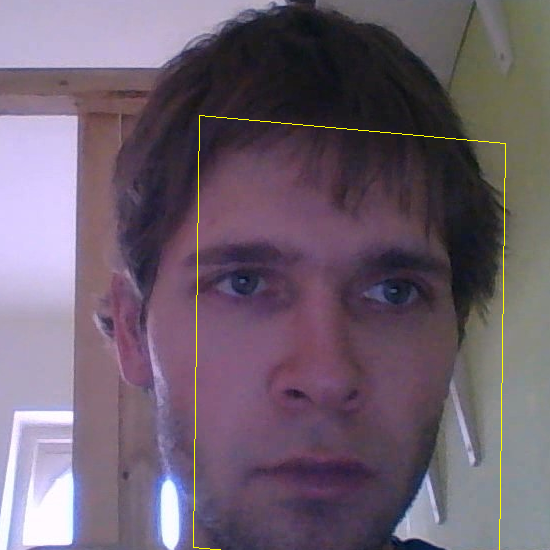
\includegraphics[width=\linewidth]{img/res-face-aff.png} \caption{Quadrangle affinity tracker.} \label{i:res-face-aff}
	\end{subfigure}
	\begin{subfigure}[b]{0.49\textwidth}
		\centering 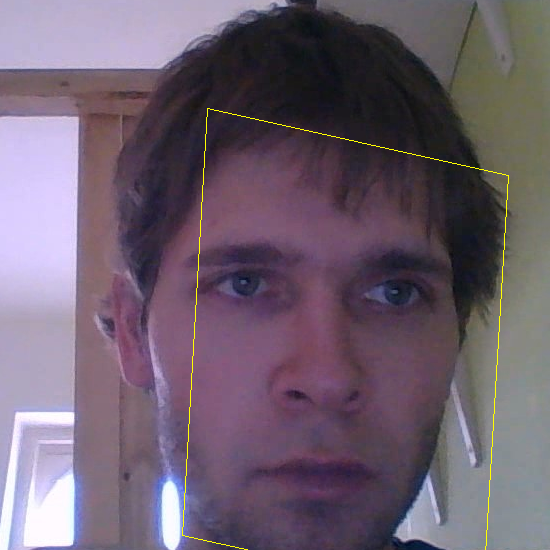
\includegraphics[width=\linewidth]{img/res-face-bary.png} \caption{Triangle affinity tracker.} \label{i:res-face-bary}
	\end{subfigure}
	\begin{subfigure}[b]{0.49\textwidth}
		\centering 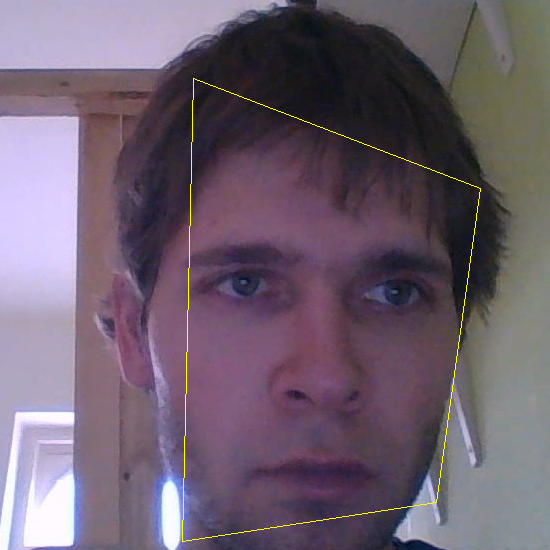
\includegraphics[width=\linewidth]{img/res-face-persp.png} \caption{Homography tracker.} \label{i:res-face-persp}
	\end{subfigure}
	\caption{Examples of the master tracker performance on two images.}\label{i:res-face}
\end{figure}

Note that in the case of the triangle affinity tracker, the area of interest is drawn as a quadrangle.
This is only a flaw in the user interface: in fact, the bottom two vertices are collapsed together to form the third vertex of a triangle.

\section{Eye tracking}

For a start, we compared the overall performance on all data available.

There are two combined trackers in addition to all the simple ones.
The one called \textit{serial} is a Hough tracker and a Limbus gradient tracker running in series, in this order.
In the tracker called \textit{serioparallel}, we replaced the simple Hough tracker with a parallel combination of Correlation, Hough, and Radial trackers.
Again, the result is refined by the Limbus gradient tracker afterwards.

\begin{table}[h]
\centering
\begin{tabular}{l@{\hspace{1.5cm}}D{.}{.}{3.2}D{.}{.}{3.2}D{.}{.}{3.2}D{.}{.}{3.2}D{.}{.}{3.2}}
\toprule
\textbf{Algorithm} & \mc{\textbf{Mean [px]}} & \mc{\textbf{Q1 [px]}} & \mc{\textbf{Q2 [px]}} & \mc{\textbf{Q3 [px]}} \\
\midrule
serial & 7.30 & 0.59 & 0.90 & 1.43 \\
hough & 8.26 & 0.98 & 1.36 & 2.02 \\
serioparallel & 11.97 & 0.75 & 1.45 & 5.67 \\
radial & 12.11 & 0.89 & 1.73 & 4.44 \\
correlation & 16.48 & 0.97 & 1.99 & 6.83 \\
bitmap & 28.55 & 3.76 & 6.54 & 13.62 \\
limbus & 35.23 & 5.77 & 10.71 & 16.67 \\
\bottomrule
\end{tabular}
\caption{Algorithm mean error and quartiles.}\label{t:algo-mean}
\end{table}

Looking at the quartiles Q1 and Q2, it seems that there are many nice cases where the algorithms perform well.
Indeed, Figure \ref{i:res-graph} shows the results of each of the trackers are sorted by distance, so that the error distribution becomes apparent.

\begin{figure}[t]
	\centering
	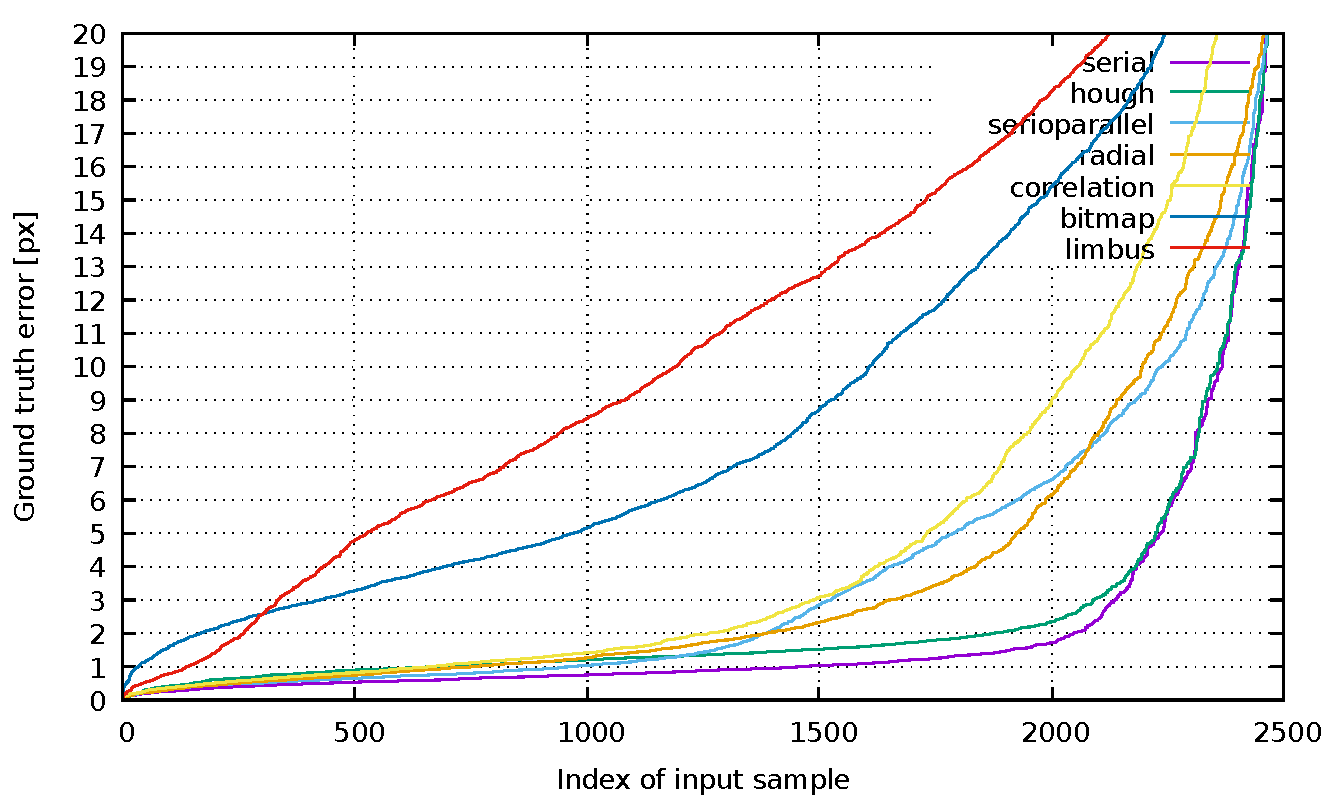
\includegraphics[width=\linewidth]{img/res-graph.pdf}
	\caption{Comparison of the eye trackers, each data row sorted by distance.} \label{i:res-graph}
\end {figure}

We evaluated the algorithms separately on each of our data sets separately.
Example images from each of these can be seen in Figure \ref{i:res-data}, and they are described in Attachment \ref{s:testingdata}.

\begin{figure}[t]
	\centering 
	\begin{subfigure}[b]{0.7\textwidth}
		\centering 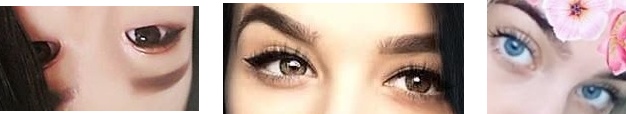
\includegraphics[width=\linewidth]{img/data-instagram.png} \caption{``Instagram" data set.} \label{i:res-data-instagram}
	\end{subfigure}
	\begin{subfigure}[b]{0.7\textwidth}
		\centering 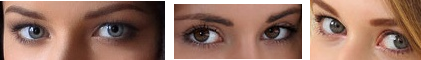
\includegraphics[width=\linewidth]{img/data-models.png} \caption{``Models" data set.} \label{i:res-data-models}
	\end{subfigure}
	\begin{subfigure}[b]{0.7\textwidth}
		\centering 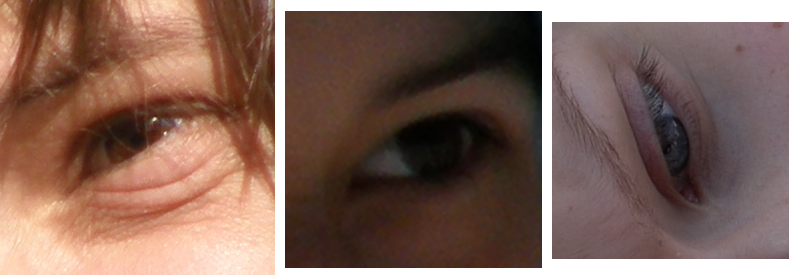
\includegraphics[width=\linewidth]{img/data-eyes.png} \caption{``Eyes" data set.} \label{i:res-data-eyes}
	\end{subfigure}
	\caption{Example files from the data sets used.}\label{i:res-data}
\end{figure}

Apparently, the simple tracker based on Circle Hough Transformation provides the best result.
Its performance can be improved on subpixel scale by adding an additional step of the Limbus gradient optimization.

It is quite disappointing that a voting scheme based on three of our trackers appears to perform worse than the best of them.

We should note that our Radial tracker is considerably slower than all the remaining ones.
On overly large-resolution images, its execution time can actually harm the overall framerate of gaze recognition.

\subsection{Failure factors}
\label{s:results-eyecovar}

Apparently, the results of eye tracking depend heavily on the qualitative aspects of each image.
For this reason, we annotated each of our testing samples in the several regards, as follows.
Each of them is evaluated on a subjective scale:
\begin{itemize}
\item \textbf{Iris} brightness:
1 (not distinguishable from the pupil) to 3 (bright blue)
\item Image \textbf{contrast}:
1 (image is hardly visible) to 3 (perfect)
\item \textbf{Glare} or reflection:
1 (not visible), 2 (only a few pixels), 3 (large)
%\item \textbf{Occlusion} by eyelids, hair and other objects:
%1 (whole iris visible) to 4 (sclera not visible)
\end{itemize}
Apart from this, each eye sample has already been labeled with the iris radius.

As expected, there is a strong correlation between many of these quantities:
\begin{table}[h!]
\centering
\begin{tabular}{l@{\hspace{1.5cm}}D{.}{.}{3.2}D{.}{.}{3.2}D{.}{.}{3.2}D{.}{.}{3.2}}
\toprule
\textbf{Algorithm} & \mc{\textbf{Radius}} & \mc{\textbf{Iris}} & \mc{\textbf{Contrast}} & \mc{\textbf{Glare}}\\
\midrule
serial & 21.44 & 0.17 & -0.14 & -0.49\\
hough & 16.68 & -0.11 & -0.09 & -0.49\\
serioparallel & 33.03 & 1.80 & 0.19 & 0.73\\
radial & 37.92 & 0.61 & 0.02 & 0.76\\
correlation & 34.09 & 3.30 & -0.06 & 1.29\\
bitmap & 72.23 & 0.74 & 0.54 & 1.43\\
limbus & 46.57 & 0.54 & 0.37 & 0.41\\
\bottomrule
\end{tabular}
\caption{Covariance of mean error wrt. image properties.}\label{t:algo-covar}
\end{table}

For completeness, we repeated this test with each of our data sets.
These detailed results are provided in tables \ref{t:algo-covar-instagram}, \ref{t:algo-covar-models} and \ref{t:algo-covar-eyes}.
The overall eye tracking performance on each of the data sets is listed in Table \ref{t:algo-mean-data}.

Clearly, the performance of the Correlation tracker is harmed by bright iris color.
This is confirmed consistently in all of the data sets.
The serioparallel tracker has been designed with this fact in mind, so that if correlation tracking fails, the remaining two votes should still provide a good estimate.
It seems that the combination technique is inefficient because it improves only few of the results.

The limbus gradient maximizer shows

\begin{table}[h]
\centering
\begin{tabular}{l@{\hspace{1.5cm}}D{.}{.}{3.2}D{.}{.}{3.2}D{.}{.}{3.2}}
\toprule
\textbf{Algorithm} & \mc{\textbf{Instagram}} & \mc{\textbf{Models}} & \mc{\textbf{Eyes}}\\
\midrule
serial            & 6.43 &6.72 & 23.98 \\
hough           & 7.52 & 7.74& 22.80 \\
serioparallel & 10.64 & 12.44& 22.40  \\
radial           & 11.37 & 11.44&  28.36 \\
correlation   & 14.18 &18.42&22.02  \\
bitmap          & 31.04 & 24.39&  45.47 \\
limbus          & 35.53 &33.50 &51.08   \\
\bottomrule
\end{tabular}
\caption{Algorithm mean error on each dataset.}\label{t:algo-mean-data}
\end{table}

\begin{table}[h]
\centering
\begin{tabular}{l@{\hspace{1.5cm}}D{.}{.}{3.2}D{.}{.}{3.2}D{.}{.}{3.2}D{.}{.}{3.2}}
\toprule
\textbf{Algorithm} & \mc{\textbf{Radius}} & \mc{\textbf{Iris}} & \mc{\textbf{Contrast}} & \mc{\textbf{Glare}}\\
\midrule
serial & 4.08 & 0.50 & -0.13 & -0.59\\
hough & 4.12 & 0.23 & -0.08 & -0.74\\
serioparallel & 14.00 & 2.06 & 0.05 & 0.80\\
radial & 11.80 & 0.81 & -0.11 & 0.77\\
correlation & 17.48 & 3.27 & -0.24 & 1.28\\
bitmap & 41.83 & 1.54 & 0.03 & 2.17\\
limbus & 19.12 & 1.06 & -0.10 & 0.89\\
\bottomrule
\end{tabular}
\caption{Error covariance on the Instagram data set.}\label{t:algo-covar-instagram}
\end{table}

\begin{table}[h]
\centering
\begin{tabular}{l@{\hspace{1.5cm}}D{.}{.}{3.2}D{.}{.}{3.2}D{.}{.}{3.2}D{.}{.}{3.2}}
\toprule
\textbf{Algorithm} & \mc{\textbf{Radius}} & \mc{\textbf{Iris}} & \mc{\textbf{Contrast}} & \mc{\textbf{Glare}}\\
\midrule
serial & 21.77 & -0.23 & -0.09 & 0.13\\
hough & 16.66 & -0.47 & -0.06 & 0.11\\
serioparallel & 34.50 & 0.95 & 0.25 & 0.76\\
radial & 31.32 & 0.29 & 0.04 & 0.85\\
correlation & 47.50 & 2.24 & 0.23 & 1.32\\
limbus & 19.90 & 0.13 & 0.29 & 0.23\\
bitmap & 55.13 & 0.78 & 0.53 & 1.32\\
\bottomrule
\end{tabular}
\caption{Error covariance on the Models data set.}\label{t:algo-covar-models}
\end{table}

\begin{table}[h]
\centering
\begin{tabular}{l@{\hspace{1.5cm}}D{.}{.}{3.2}D{.}{.}{3.2}D{.}{.}{3.2}D{.}{.}{3.2}}
\toprule
\textbf{Algorithm} & \mc{\textbf{Radius}} & \mc{\textbf{Iris}} & \mc{\textbf{Contrast}} & \mc{\textbf{Glare}}\\
\midrule
serial & 99.61 & -1.39 & -2.67 & 1.51\\
hough & 56.33 & -1.97 & -2.16 & 2.54\\
serioparallel & 194.48 & 3.59 & 0.44 & 4.07\\
radial & 301.92 & 0.13 & -0.37 & 7.31\\
correlation & 109.67 & 5.91 & -0.99 & 2.78\\
limbus & 524.95 & 2.16 & 4.79 & 4.64\\
bitmap & 392.63 & 4.26 & 3.33 & 3.20\\
\bottomrule
\end{tabular}
\caption{Error covariance on the Eyes data set.}\label{t:algo-covar-eyes}
\end{table}

